\documentclass[a4paper,11pt]{exam}
\printanswers % pour imprimer les réponses (corrigé)
%\noprintanswers % Pour ne pas imprimer les réponses (énoncé)
\addpoints % Pour compter les points
% \noaddpoints % pour ne pas compter les points
%\qformat{\textbf{\thequestion ) } }
\qformat{\textbf{\thequestion )} \textit{(\thepoints)} \\  } % Pour définir le style des questions (facultatif)
\usepackage{color} % définit une nouvelle couleur
\shadedsolutions % définit le style des réponses
% \framedsolutions % définit le style des réponses
\definecolor{SolutionColor}{rgb}{0.8,0.9,1} % bleu ciel
\renewcommand{\solutiontitle}{\noindent\textbf{Solution:}\par\noindent} % Définit le titre des solutions




\makeatletter

\def\maketitle{{\centering%
	\par{\huge\textbf{\@title}}%
	\par{\@date}%
	\par}}

\makeatother

\lhead{NOM Pr\'enom :}
\rhead{\textbf{Les r\'eponses doivent \^etre justifi\'ees}}
\cfoot{\thepage / \pageref{LastPage}}


%\usepackage{../../pas-math}
%\usepackage{../../moncours}


%\usepackage{pas-cours}
%-------------------------------------------------------------------------------
%          -Packages nécessaires pour écrire en Français et en UTF8-
%-------------------------------------------------------------------------------
\usepackage[utf8]{inputenc}
\usepackage[frenchb]{babel}
\usepackage[T1]{fontenc}
\usepackage{lmodern}
\usepackage{textcomp}



%-------------------------------------------------------------------------------

%-------------------------------------------------------------------------------
%                          -Outils de mise en forme-
%-------------------------------------------------------------------------------
\usepackage{hyperref}
\hypersetup{pdfstartview=XYZ}
%\usepackage{enumerate}
\usepackage{graphicx}
\usepackage{multicol}
\usepackage{tabularx}
\usepackage{multirow}


\usepackage{anysize} %%pour pouvoir mettre les marges qu'on veut
%\marginsize{2.5cm}{2.5cm}{2.5cm}{2.5cm}

\usepackage{indentfirst} %%pour que les premier paragraphes soient aussi indentés
\usepackage{verbatim}
\usepackage{enumitem}
\usepackage[usenames,dvipsnames,svgnames,table]{xcolor}

\usepackage{variations}

%-------------------------------------------------------------------------------


%-------------------------------------------------------------------------------
%                  -Nécessaires pour écrire des mathématiques-
%-------------------------------------------------------------------------------
\usepackage{amsfonts}
\usepackage{amssymb}
\usepackage{amsmath}
\usepackage{amsthm}
\usepackage{tikz}
\usepackage{xlop}
%-------------------------------------------------------------------------------



%-------------------------------------------------------------------------------


%-------------------------------------------------------------------------------
%                    - Mise en forme avancée
%-------------------------------------------------------------------------------

\usepackage{ifthen}
\usepackage{ifmtarg}


\newcommand{\ifTrue}[2]{\ifthenelse{\equal{#1}{true}}{#2}{$\qquad \qquad$}}

%-------------------------------------------------------------------------------

%-------------------------------------------------------------------------------
%                     -Mise en forme d'exercices-
%-------------------------------------------------------------------------------
%\newtheoremstyle{exostyle}
%{\topsep}% espace avant
%{\topsep}% espace apres
%{}% Police utilisee par le style de thm
%{}% Indentation (vide = aucune, \parindent = indentation paragraphe)
%{\bfseries}% Police du titre de thm
%{.}% Signe de ponctuation apres le titre du thm
%{ }% Espace apres le titre du thm (\newline = linebreak)
%{\thmname{#1}\thmnumber{ #2}\thmnote{. \normalfont{\textit{#3}}}}% composants du titre du thm : \thmname = nom du thm, \thmnumber = numéro du thm, \thmnote = sous-titre du thm

%\theoremstyle{exostyle}
%\newtheorem{exercice}{Exercice}
%
%\newenvironment{questions}{
%\begin{enumerate}[\hspace{12pt}\bfseries\itshape a.]}{\end{enumerate}
%} %mettre un 1 à la place du a si on veut des numéros au lieu de lettres pour les questions 
%-------------------------------------------------------------------------------

%-------------------------------------------------------------------------------
%                    - Mise en forme de tableaux -
%-------------------------------------------------------------------------------

\renewcommand{\arraystretch}{1.7}

\setlength{\tabcolsep}{1.2cm}

%-------------------------------------------------------------------------------



%-------------------------------------------------------------------------------
%                    - Racourcis d'écriture -
%-------------------------------------------------------------------------------

% Angles orientés (couples de vecteurs)
\newcommand{\aopp}[2]{(\vec{#1}, \vec{#2})} %Les deuc vecteurs sont positifs
\newcommand{\aopn}[2]{(\vec{#1}, -\vec{#2})} %Le second vecteur est négatif
\newcommand{\aonp}[2]{(-\vec{#1}, \vec{#2})} %Le premier vecteur est négatif
\newcommand{\aonn}[2]{(-\vec{#1}, -\vec{#2})} %Les deux vecteurs sont négatifs

%Ensembles mathématiques
\newcommand{\naturels}{\mathbb{N}} %Nombres naturels
\newcommand{\relatifs}{\mathbb{Z}} %Nombres relatifs
\newcommand{\rationnels}{\mathbb{Q}} %Nombres rationnels
\newcommand{\reels}{\mathbb{R}} %Nombres réels
\newcommand{\complexes}{\mathbb{C}} %Nombres complexes


%Intégration des parenthèses aux cosinus
\newcommand{\cosP}[1]{\cos\left(#1\right)}
\newcommand{\sinP}[1]{\sin\left(#1\right)}


%Probas stats
\newcommand{\stat}{statistique}
\newcommand{\stats}{statistiques}
%-------------------------------------------------------------------------------

%-------------------------------------------------------------------------------
%                    - Mise en page -
%-------------------------------------------------------------------------------

\newcommand{\twoCol}[1]{\begin{multicols}{2}#1\end{multicols}}


\setenumerate[1]{font=\bfseries,label=\textit{\alph*})}
\setenumerate[2]{font=\bfseries,label=\arabic*)}


%-------------------------------------------------------------------------------
%                    - Elements cours -
%-------------------------------------------------------------------------------




\usepackage{tabu}

%\usepackage{fullpage}
\author{\ }
\date{11 Avril 2019}
\title{$1^{ère}$ $ST_2S$ : DS num\'ero 4}


\begin{document}
%	\usepackage{fancyhdr}
%	
%	\pagestyle{fancy}
%	\fancyhf{}
	%\rhead{Share\LaTeX}

	\maketitle



\section{Débouchés post bac (8 points)}

Un lycée lance une enquête pour connaître les poursuites d'études suivies par les élèves reçu au bac ST2S en 2006.
Pour les 54 élèves lauréats, on a obtenu les seuls renseignements suivants :
\begin{itemize}
	\item 14 filles et 1 garçon sont en instituts de soins en soin infirmiers (IFSI);
	\item 18 filles et 3 garçons sont en BTS ESF ;
	\item 12 filles sont entrées dans la vie active ;
	\item aucun garçon n'est entré dans la vie active ;
	\item tous les garçons ont répondu.
\end{itemize}

\begin{questions}
	\question[2] Compléter le tableau suivant :
	
	\begin{center}		
		\begin{tabular}{|@{\ \ \ }l@{\ \ \ }|@{\ \ \ }c@{\ \ \ }|@{\ \ \ }c@{\ \ \ }|@{\ \ \ }c@{\ \ \ }|}
\hline
                            & \textbf{Fille(s)} & \textbf{Garçon(s)} & \textbf{Total} \\ \hline
\textbf{En IFSI}            &                   &                    & 15             \\ \hline
\textbf{En BTS ESF}         &                   &                    &                \\ \hline
\textbf{Dans la vie active} &                   &                    &                \\ \hline
\textbf{Pas de réponse}     &                   &                    &                \\ \hline
\textbf{Total}              &                   &                    & 54             \\ \hline
\end{tabular}
	\end{center}
	
	%\question Calculer le pourcentage de lauréats ayant répondu à l'enquête. Arrondir le résultat à \num{0.1} \% près.
	
	\textit{Dans les questions suivantes, les résultats seront donnés sous forme décimale à \num{0.01} près.}
	\question On choisit un élève au hasard parmi les 54 lauréats et on considère les événements suivants :
	\begin{itemize}
		\item $A$ : << Le lauréat est un garçon >>;
		\item $B$ : << Le lauréat a répondu qu'il est en institut de formation en soins infirmiers >>;
		\item $C$ : << Le lauréat est un garçon  en BTS ESF>>;
		\item $B$ : << Le lauréat est une filles qui a répondu être en institut de formation en soins infirmiers >>.
	\end{itemize}

		\begin{parts}
			\part[1] \'Ecrire l'événement $D$ à l'aide des événements $A$ et $B$.
			\part[2] Calculer la probabilité de chacun des événements $A$, $B$, $C$ et $D$.
			\part[1] Décrire l'événement $\bar{A} \cup B$ à l'aide d'une phrase. Calculer la probabilité de cet événement.
		\end{parts}
	
	\question[2] On suit au hasard un lauréat qui a répondu être en institut de formations en soins infirmiers. Calculer la probabilité que ce soit une fille. 
\end{questions}

\section{Le self de la cantine (8 points)}

Une cantine propose en self-service un choix de deux hors-d'\oe uvre, trois plats chauds et trois desserts. Deux plateaux repas sont dit identiques lorsqu'ils sont composés du même hors d'\oe uvre, du même plat chaud et du même dessert.

\begin{questions}
	\question[4] Combien de plateaux repas différents peut-on constituer dans cette cantine ? Donner tous les choix possibles. 
	
	
	On pourra noter les hors d'\oe uvre $H$, les plats chauds $P$ et les desserts $D$. Par exemple le choix $H_2P_1D_1$ correspond à un plateau composé du hors d'\oe uvre n°2, du plat chaud n°1 et du dessert n°1. 
	
	\question 
		\begin{parts}
			\part[1] Un(e) camarade compose au hasard un plateau repas pour vous un jour où un seul plateau vous fait envie. Quelle est, sous forme de fraction, la probabilité que ce choix vous convienne, en supposant que tous les plateaux repas sont équiprobables ?
			
			\part[1] Même question un jour où vous aimez tout sauf un des plats chauds.
			
			\part[1] Même question un jour où seul un des desserts ne vous convient pas mais tout le reste vous plait. 
		\end{parts}
	
	\question[1] \`A la demande des élèves, il est décidé qu'un plat supplémentaire sera préparé. Ce plat doit-il être un hors d'\oe uvre, un plat chaud ou un dessert pour que les élèves aient un maximum de choix pour leur plateaux repas. 
\end{questions}

\section{Un jeu de cartes (5 points)}

On tire au hasard une carte dans un jeu de trente-deux. Les trente-deux événements élémentaires sont équiprobables.

\begin{questions}
	
	
	\question[1] Donner deux événements incompatibles.
	\begin{solution}
		Les événements <<la carte tirée est un c\oe ur>> et <<la carte tirée est un pique>> sont incompatibles.
	\end{solution}
	
	\question Les événements $A$ et $B$ sont-ils indépendants ?
	
		\begin{parts}
			\part[2] $A$ : <<la carte tirée est une dame >>; $B$ : <<la carte tirée est noire>>.
			
			\begin{solution}
				\begin{eqnarray}
					P(A) &=& \dfrac{4}{32} = \dfrac{1}{8} \\
					P(B) &=& \dfrac{1}{2}\\
					P(A \cap B) &= & \dfrac{2}{32} = \dfrac{1}{16}\\
					P(A) \times P(B) &=& \dfrac{1 \times 1}{8 \times 2} = \dfrac{1}{16}
				\end{eqnarray}
				
				On a $P(A\cap B)  = P(A) \times P(B)$, donc les événements $A$ et $B$ sont indépendants.
			\end{solution}
			
			\part[2] $A$ : <<la carte tirée est une dame >>; $B$ : <<la carte tirée est une figure>>.
			
			\begin{solution}
				\begin{eqnarray}
				P(A) &=& \dfrac{4}{32} = \dfrac{1}{8} \\
				P(B) &=& \dfrac{12}{32} = \dfrac{3}{8}\\
				P(A \cap B) &= & \dfrac{4}{32} = \dfrac{1}{8}\\
				P(A) \times P(B) &=& \dfrac{1 \times 3}{8 \times 8} = \dfrac{3}{64}
				\end{eqnarray}
				
				On a $P(A\cap B)  \neq P(A) \times P(B)$, donc les événements $A$ et $B$ ne sont pas indépendants.
			\end{solution}
		\end{parts}
\end{questions} 



%\section{Un vrai-faux (6 points)}

Répondez par VRAI ou FAUX aux affirmations suivantes. Une justification est demandée lorsque la réponse est FAUX, aucune justification n'est demandée lorsque la réponse est VRAI.

\begin{questions}
	\question[1] Pour une série ordonnée comptant 512 nombres, la médiane n'existe pas car 512 est pair.
	
	\question[1] En France, le salaire mensuel moyen s'élève à \num{2500} € et le salaire mensuel médian s'élève à \num{1600} €. Plus de 50 \% des salariés gagnent moins de \num{2500} € par mois.
	
	\question[1] Le couple médiane et écart interquartile est peu sensible aux valeurs extrêmes de la série statistique.
	
	\question[1] La moyenne rend compte de la dispersion de la série statistique.
	
	\question[1] Si une série statistique compte 10 valeurs, les quartiles sont toujours des valeurs de la série.
	
	\question[1] On donne la série : 1 ; 2 ; 3 ; 4 ; 4 ; 4 ; 5 ; 8 ; 9 ; 10. L'écart interquartille est 5.
\end{questions}
%\section{La répartition des médecins}

\subsection{Actifs et retraités actifs}

Le diagramme de la figure \ref{fig:repartition} donne la répartition des médecins actifs inscrits au conseil de l'ordre en 2011.

\begin{figure}{h}
	\begin{center}
		%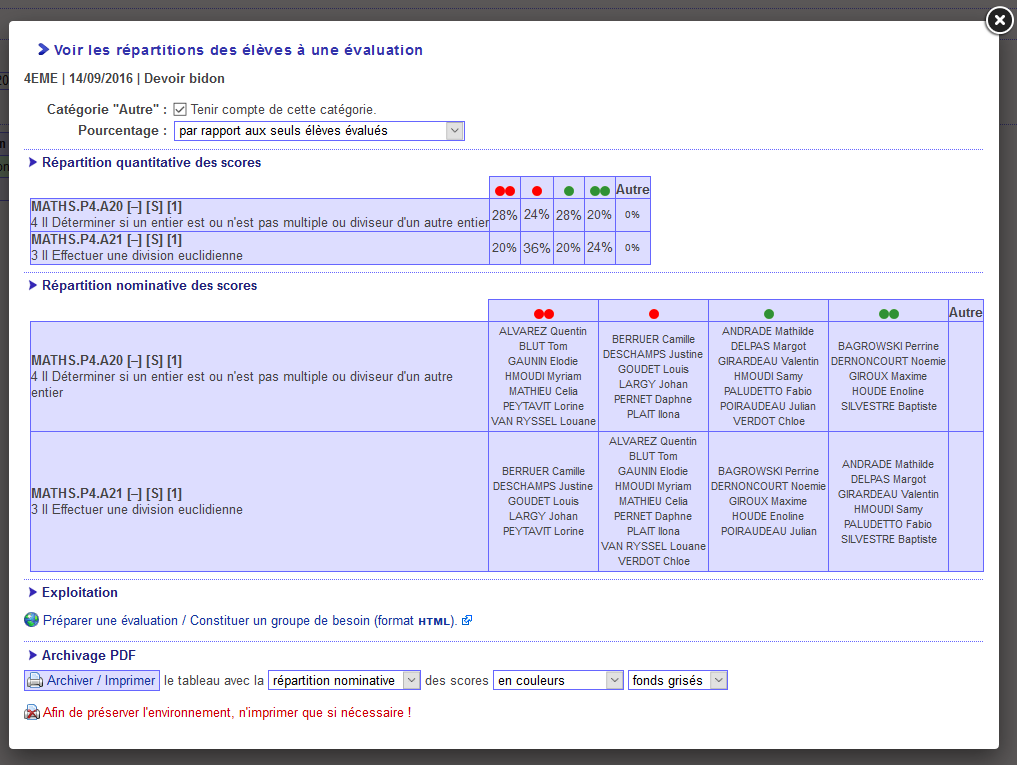
\includegraphics[scale=0.5]{repartition}
		\caption{Répartition des médecins actifs en 2011}
		\label{fig:repartition}
	\end{center}
\end{figure}


\begin{questions}
	\question Quel pourcentage de l'ensemble des médecins actifs représentent les médecins retraités en 2011 ? Arrondir à \num{0.1} \%.
	
	\question Déterminer le nombre de médecins actifs non retraités en 2010.
	
	\question Déterminer le nombre de médecins actifs retraités en 2010.
	
	\question Déterminer l'augmentation en pourcentage du nombre de médecins actifs entre 2010 et 2011. Arrondir à \num{0.1} \%.
	
\end{questions}

\subsection{Les modes d'exercice}

\begin{questions}
	
	\question Le diagramme de la figure \ref{fig:mode_exercice1} donne la répartition des modes d'exercice des médecins actifs inscrits au conseil de l'ordre en 2011. Déterminer l'effectif pour chacun des modes d'exercice.
	
	\begin{figure}{h}
		\begin{center}
			%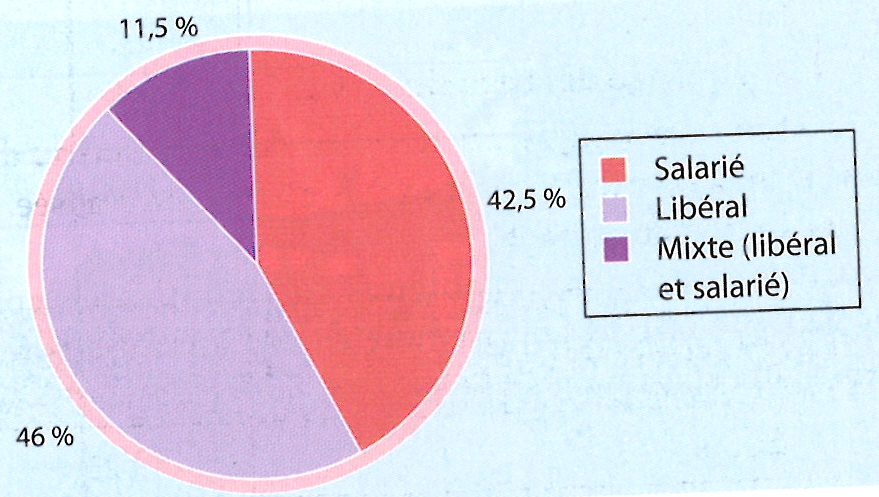
\includegraphics[scale=0.5]{mode_exercice1}
			\caption{Modes d'exercice des médecins actifs en 2011}
			\label{fig:mode_exercice1}
		\end{center}
	\end{figure}
	
	\question Le diagramme de la figure \ref{fig:mode_exercice1} donne la répartition des modes d'exercice des \num{27774} médecins de moins de 40 ans en 2011. Donner l'effectif pour chacun des modes d'exercice.
	
	\begin{figure}{h}
		\begin{center}
			%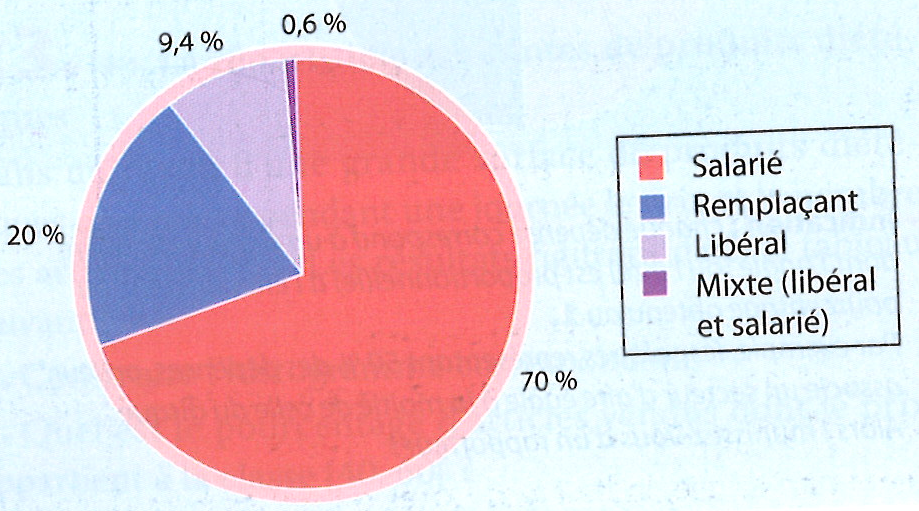
\includegraphics[scale=0.5]{mode_exercice2}
			\caption{Modes d'exercice des moins de 40 ans en 2011}
			\label{fig:mode_exercice2}
		\end{center}
	\end{figure}
	
	
	\question Quel commentaire peut-on faire sur les modes d'exercice des médecins actifs ?
\end{questions}

%\newpage

%\section{Implantation d'éoliennes \textit{(12,5 points)}}

Les parties \ref{part:site_M} et \ref{part:site_F} sont indépendantes.

Après étude, les autorités d'une ile isolée ont décidé d'installer une éolienne pour répondre aux besoins énergétiques de leur communauté. L'éolienne choisie fonctionne lorsque le vent atteint au moins 8 n\oe uds et il faut l'arrêter lorsque le vent atteint ou dépasse les 48 n\oe uds. 

\subsection{\'Etude des vitesses du vent sur le site M \textit{(7 points)}}\label{part:site_M}

Les autorités décident de mesurer pendant un mois, à l'aide d'un anémomètre, la vitesse du vent sur le site M, au sommet d'une montagne. Une mesure est effectuée chaque jour.

Les résultats obtenus sont présentés dans la tableau de la figure \ref{tab:site_M} (le mois comporte 30 jours) :

\begin{figure}[h]
	\begin{center}
		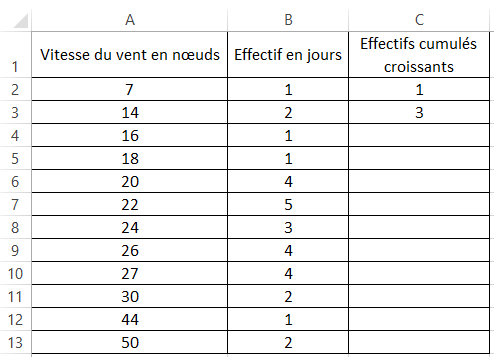
\includegraphics[scale=0.8]{eoliennes2}
	\end{center}
\caption{\'Etude de la vitesse du vent sur le site M}
\label{tab:site_M}
\end{figure}

On peut y lire que la vitesse de 22 n\oe uds a été mesurée 5 jours.

\begin{questions}
	\question[3]
		\begin{parts}
			\part[1] Compléter le tableau.
			
			\part[1] Donner une formule à placer en \textbf{\texttt{C3}} permettant, par recopie vers le bas, de calculer les effectifs cumulés croissants des jours du mois étudié.
			
			\part[1] Calculer le pourcentage des jours du mois étudié où l'éolienne ne produirait pas d'électricité. 
		\end{parts}
	
	
	\question[2] Déterminer l'étendue, la médiane, les quartiles et l'écart interquartile de cette série statistique.
	
	\question[1] On appelle premier décile (noté $D_1$) la plus petite valeur de la vitesse du vent, telle qu'au moins 10 \% des valeurs de la série sont inférieures ou égales à $D_1$. On appelle neuvième décile (noté $D_9$) la plus petite valeur, telle qu'au moins 90 \% des valeurs de la série lui sont inférieures ou égales.
	\begin{parts}
		\part[\half] Expliquer pourquoi $D_1$ = 14.
		\part[\half] Déterminer $D_9$.
	\end{parts} 
	
\end{questions}

\subsection{\'Etude des vitesses du vent sur le site F \textit{(2 points)}}\label{part:site_F}

Un emplacement sur une falaise, appelé site F, a également été retenu. Le même mois que le site M, on a mesuré les vitesses du vent sur le site F.

La série des mesures effectuée est dans le diagramme en boite de la figure \ref{fig:comparaison}. Les extrémités du diagramme correspondent aux premiers et neuvième déciles.

\begin{questions}
	
	\question[1] Lire sur le graphique les quartiles de cette nouvelle série.
	
	\question[1] Calculer l'écart interquartile.
\end{questions}

\begin{figure}[h]
	\begin{center}
		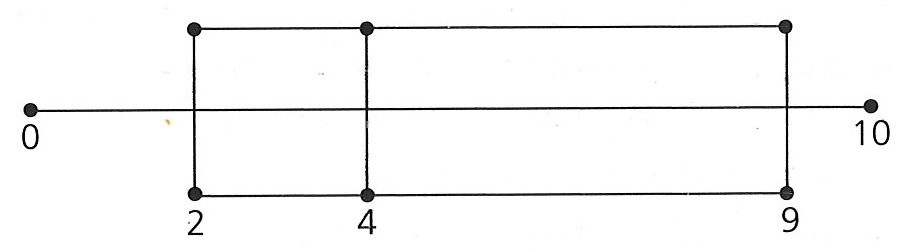
\includegraphics[scale=1.2]{moustache}
	\end{center}
	\caption{Coparaison de la vitesse du vent sur les deux sites}
	\label{fig:comparaison}
\end{figure}

\subsection{Comparaison des sites \textit{(3,5 points)}}\label{part:comp}

\begin{questions}
	\question[1\half] Représenter au-dessous du diagramme en boite fourni figure \ref{fig:comparaison}, celui de la série correspondant au site M. Prendre comme extrémités les premier et neuvième déciles.
	
	\question[2] En comparant les diagrammes, sachant qu'une éolienne a un rendement optimal aux alentours de 23 n\oe uds, quel site paraît le plsu intéressant pour l'installation de l'éolienne ? Argumenter la réponse. 
\end{questions}
	\label{LastPage}
	

\end{document}